\documentclass[t,compress]{beamer}
\usetheme{Singapore}

\sloppy
%\usepackage[scaled]{helvet}
%\usepackage{eulervm}

\usepackage{multicol}

\usepackage{fp-eval}
\usepackage{hyperref}
\usepackage{fancyvrb}
\usepackage{pstricks,pst-node,pst-tree,multido}
\usepackage{graphicx}

\usepackage{alltt}


\newcommand{\bframe}[1]{\begin{frame}[fragile]{#1}}

\newcommand{\bbnf}{\begin{center}\begin{tabular}{rcl}}
\newcommand{\bnf}[2]{#1 & ::= & #2 \\}
\newcommand{\ebnf}{\end{tabular}\end{center}}

\newcommand{\myskip}{\vspace{-1em}\hrulefill}
\newcommand{\myrule}[1]{\vspace{-1ex}\centerline{\rule{#1cm}{1pt}}}
\newcommand{\myline}[1]{\centerline{#1}}
\newcommand{\bkt}[1]{\ensuremath{\langle\mbox{#1}\rangle}}
\newcommand{\br}{\mbox{~}|\mbox{~}}

\definecolor{orange}{rgb}{1,.5,0}
\definecolor{pink}{rgb}{1,.75,.75}
\definecolor{ltblue}{rgb}{.75,.75,1}

\newcommand{\be}{\begin{eqnarray*}}
\newcommand{\ee}{\end{eqnarray*}}
\newcommand{\bi}{\begin{itemize}}
\newcommand{\ei}{\end{itemize}}

\newcommand{\grph}[2]{\centerline{\includegraphics[scale=#1]{#2}}}

\AtBeginSection[]
{
\bframe{Outline}
\tableofcontents[currentsection]
\end{frame}
}

\title{Raven Notes}
\author{CSCI 321}
\institute{Based on {\em Programming Game AI by Example}, Buckland}

\begin{document}%\small

\bframe{~}
\titlepage
\end{frame}

\bframe{Raven}

\grph{0.333}{ravenscreenshot.eps}

\end{frame}

\bframe{Raven Game Class}
\bi
\item Map
\item Bots
\item Projectiles
\item Path manager
\item Grave markers
\ei

\end{frame}

\bframe{Raven Map Class}
\bi
\item Walls
\item Trigger system
\item Spawn points
\item Doors
\item Nav graph
\item Space partition
\ei

\end{frame}

\bframe{Raven Weapons and Projectiles}
\bi
\item The Blaster
\item The Shotgun
\item The Rocket Launcher
\item The Railgun
\ei
\end{frame}

\bframe{Trigger examples in games}
\bi
\item Step on a pressure plate
\item Dead guard notifies other guards
\item Shooting a gun activates a noise trigger
\item Determine if a player has tried something three times
\item Wounded enemies leave a trail of blood
\ei
\end{frame}

\bframe{Raven Triggers}
\bi
\item Respawning
\item Givers
\bi \item Weapon \item Health \ei
\item Limited lifetime
\bi \item Sound \ei
\ei
\end{frame}

\bframe{AI design}
\bi
\item Weapon handling and movement independent
\item Predict enemy's movement
\item Choose appropriate weapon
\item Select best weapon
\item Aim slow weapons
\item Select a single target from a group
\item Perception
\bi \item Visible \item Noisy \ei
\item Perception memory
\item Planning
\ei
\end{frame}

\bframe{Raven AI Overview}
\bi
\item Decision making
\bi \item Attack \item Find health \item Chase target \ei
\item Movement
\bi \item Steering \ei
\item Path planning
\ei
\end{frame}

\bframe{Perception: Bots too aware}
Sensory omnipotence
\bi
\item Eyes behind heads
\item See you in the dark
\item See you behind obstacles
\ei
Solution:  better programming
\end{frame}

\bframe{Perception: Bots too unaware}
Selective sensory nescience
\bi
\item Set off a bomb behind them
\item Leave a corpse seen by the next guard
\item Forget about you once out of sight
\item Forget about you if they turn their head
\ei
Solution:  short-term memory

\end{frame}

\bframe{Weapon Handling}
\bi
\item Fuzzy logic for selection
\item Aim using steering for slow weapons
\ei

\end{frame}

\bframe{Weapon Handling Not Perfect}
\bi 
\item Selection 
\item Aiming 
\item Fire rate
\item Some bots {\em always} miss the first shot
\item Lower skill when player's health is low
\ei
\end{frame}

\bframe{Updating}
\bi
\item Not everything every cycle:
\bi
\item Weapon selection
\item Visible opponent recognition
\item $A^*$ path planning
\ei
\ei

\end{frame}

\bframe{Tile Based Games}

\grph{0.4}{starcraft.eps}

\end{frame}


\bframe{Sparse Graphs---Points of Visibility}

\grph{0.333}{sparsegraph.eps}

Use expanded geometry to generate automatically.

\end{frame}

\bframe{Navigation Meshes}

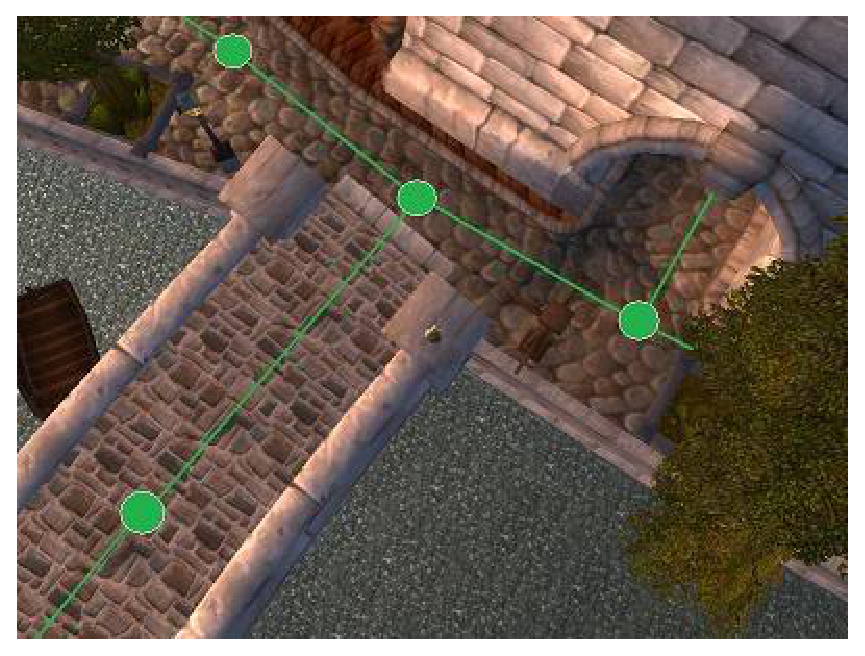
\includegraphics[scale=0.4]{Stormwind_waypoints.eps}
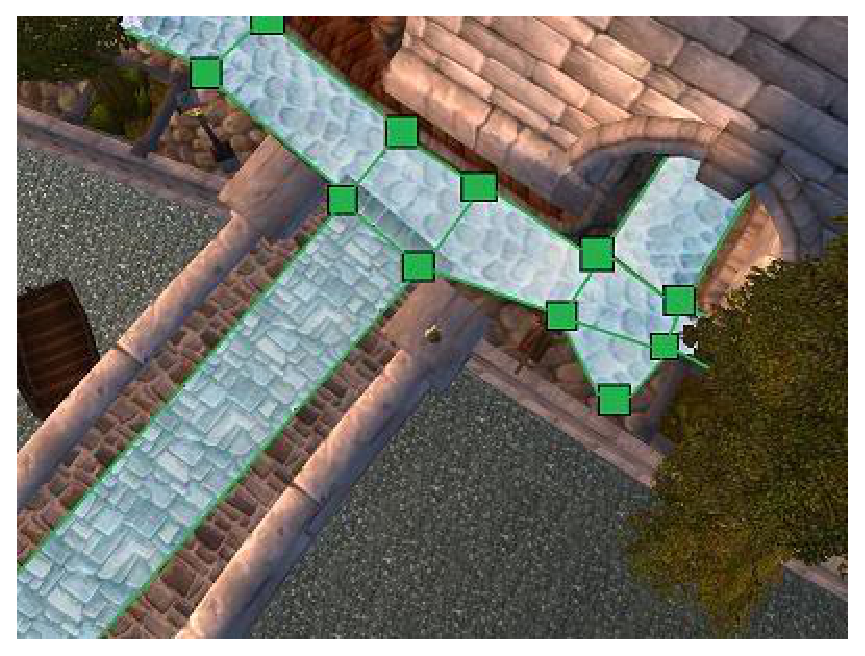
\includegraphics[scale=0.4]{Stormwind-NavMesh.eps}

\end{frame}

\bframe{Bot:  move from $x$ to $y$}
\bi
\item Algorithm:
\bi
\item Find $A$: closest graph node to $x$
\item Find $B$: closest graph node to $y$
\item Search for least cost from $A$ to $B$
\item Move to $A$
\item Follow path
\item Move to $B$
\ei
\item Problems:
\bi
\item Can be invisible points in coarse graph.
\item Coarse graph can result in poor paths.
\item Problems getting from $A$ to $x$
\ei
\ei
\end{frame}

\bframe{Fine Graph}

\grph{0.333}{finegraph.eps}

Can be built automatically with flood fill.

\end{frame}

\bframe{Spatial partitioning}

\bi
\item Need to find closest visible node.
\item Partition space.
\item Time goes from $O(n^2)$ in number of nodes to $O(d)$ in {\em
  density } of nodes, which is usually constant.
  \ei
\end{frame}

\bframe{Path finding to an item type}
\bi
\item $A^*$ good if we know the destination.
\item Finding the shortest path to the nearest ammo (on shortest path)?
\item Can use Euclidean distance and then $A^*$.
\item Dijkstra's algorithm better if there are {\em many} items.
\ei
\end{frame}

\bframe{Path smoothing}

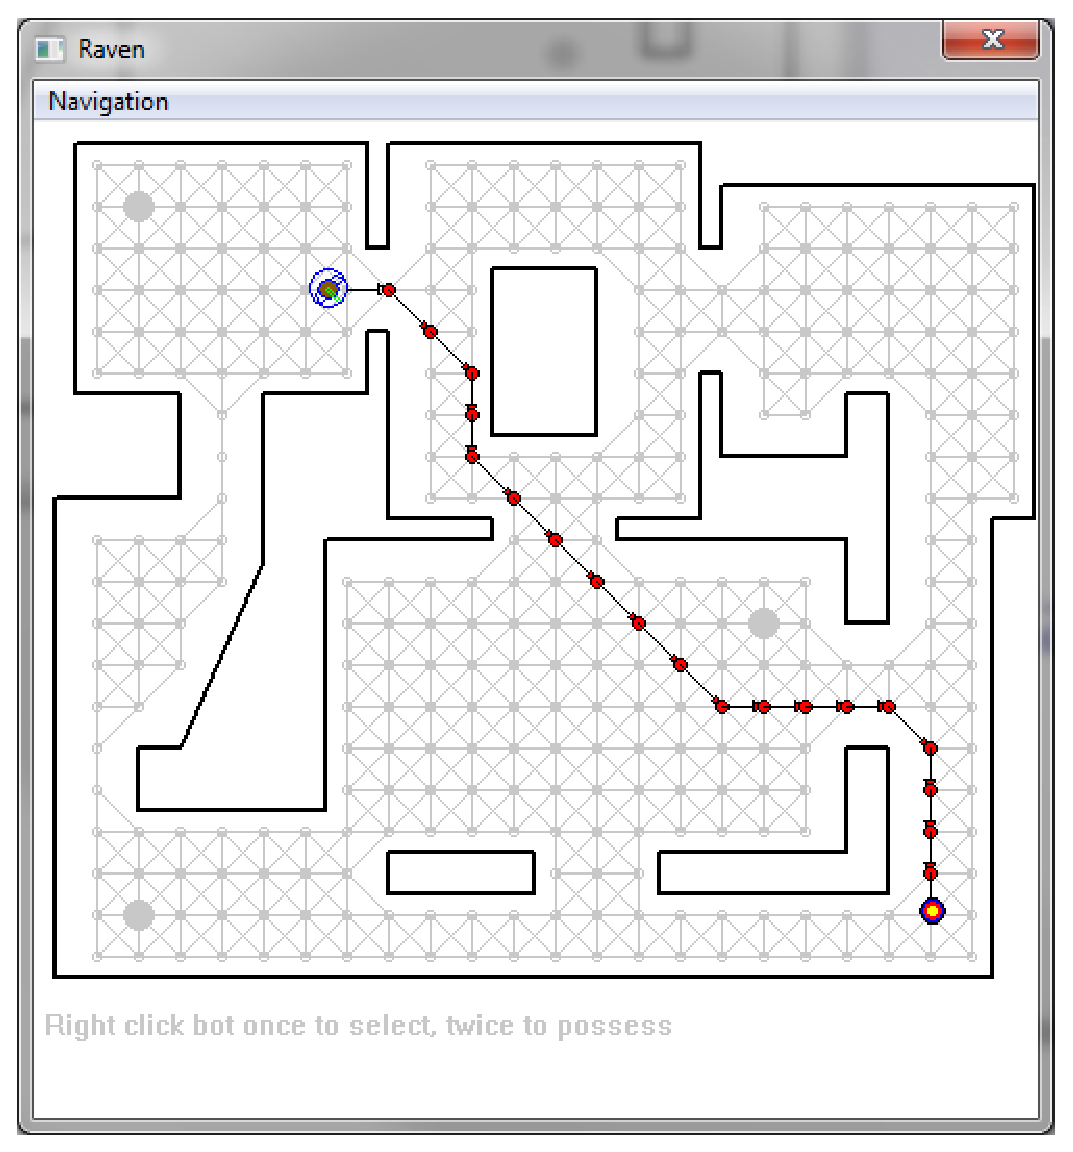
\includegraphics[scale=0.33]{unsmoothedpath.eps}
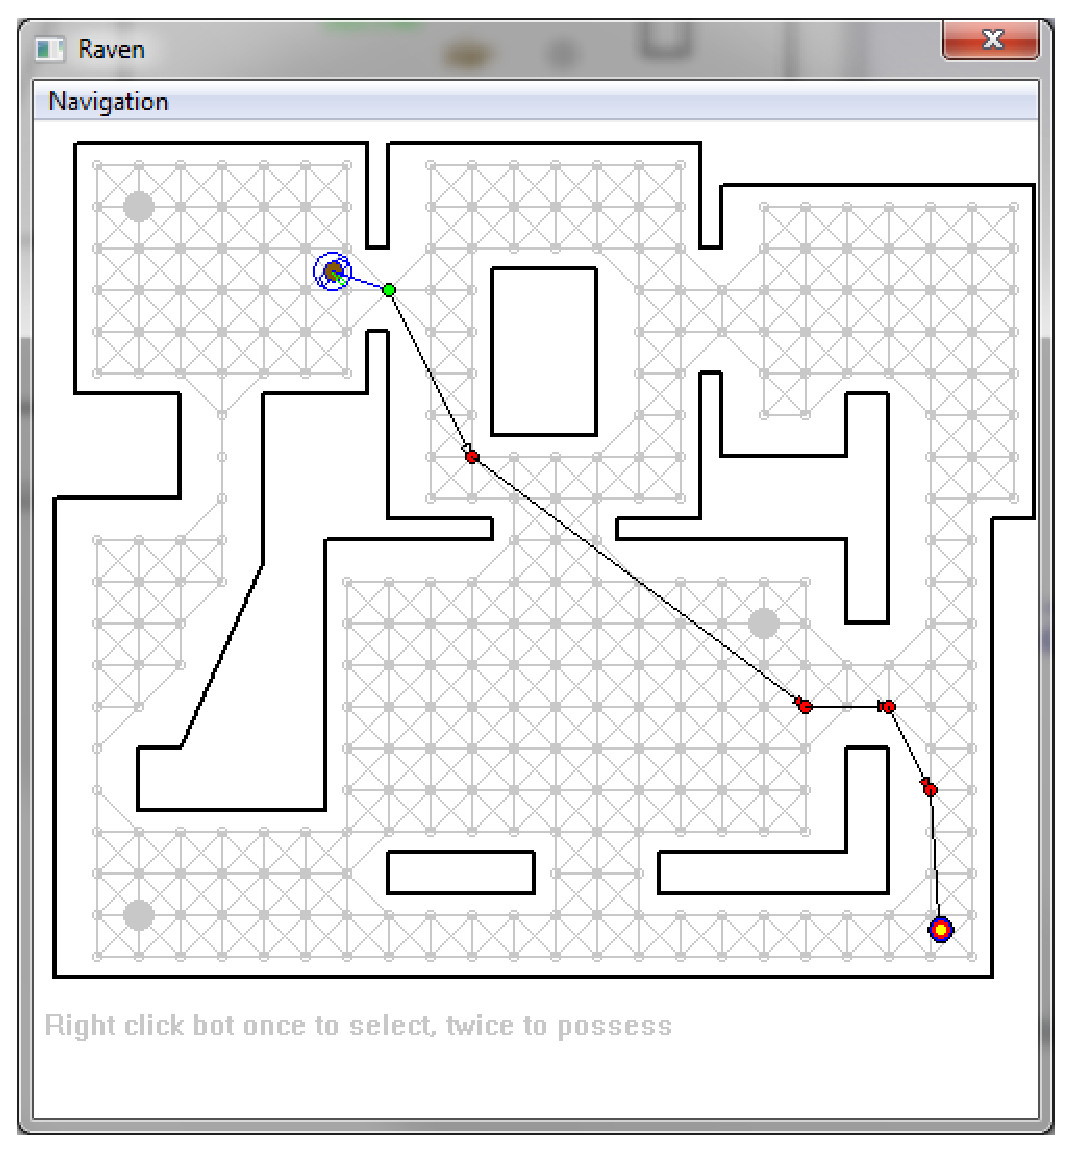
\includegraphics[scale=0.33]{smoothedpath.eps}

\end{frame}

\bframe{Precompute all shortest paths}
\begin{multicols}{2}
\begin{psmatrix}\small
\circlenode{A}{A} && \circlenode{E}{E}\\
  & \circlenode{B}{B}  \\
\circlenode{C}{C} && \circlenode{D}{D} \\
\ncline{A}{E}^{5}
\ncline{A}{B}^{3}
\ncline{A}{C}<{2}
\ncline{B}{D}^{1}
\ncline{D}{E}>{2}
\ncline{C}{B}^{3.5}
\end{psmatrix}
\columnbreak
\begin{tabular}{c|ccccc}
  & A & B & C & D & E \\\hline
A & A & B & C & B & E \\
B & A & B & C & D & D \\
C & A & B & C & B & B \\
D & B & B & B & D & E \\
E & A & D & D & D & E 
\end{tabular}
\end{multicols}

Can be augmented with total path costs.

\end{frame}

\bframe{Time Sliced Path Search}
\bi
\item Don't do searches all at once.
\item Break them up into slices.
\item Bots must avoid twiddling thumbs:
  \bi
  \item {\bf Seek} in meantime.
    \bi 
    \item Must use path smoothing.
    \ei
  \item Use modified $A^*$ to return partial results.
  \ei
\ei
\end{frame}

\bframe{Hierarchical path finding}

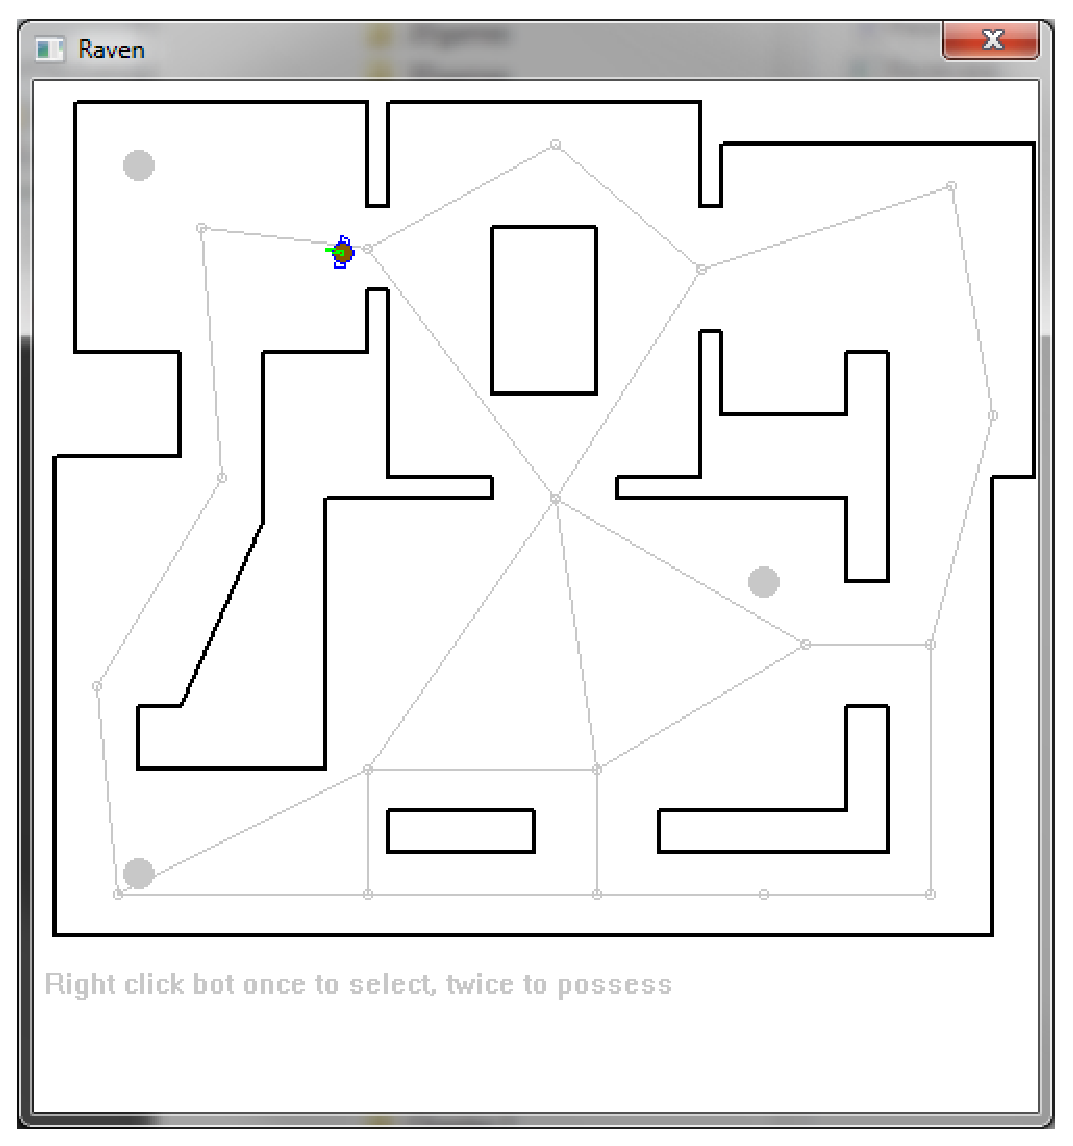
\includegraphics[scale=0.33]{sparsegraph.eps}
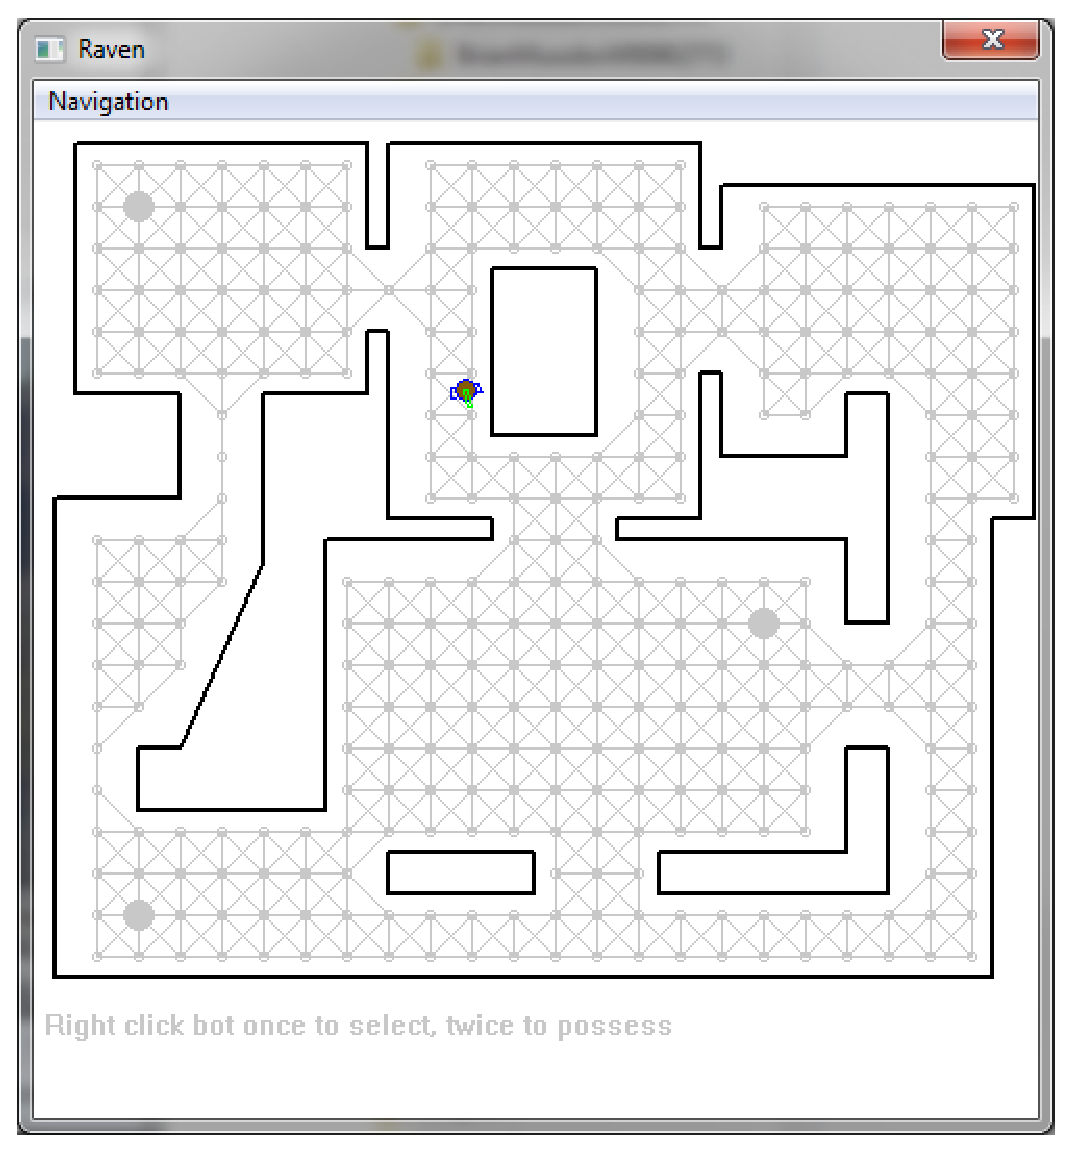
\includegraphics[scale=0.33]{finegraph.eps}

\end{frame}


\bframe{Bots getting stuck}

\grph{0.33}{botsstuck.eps}
\end{frame}

\end{document}
